% Chapter 2

\chapter{Introducción a las antenas polarimétricas} % Chapter title
\label{ch:phasedArray}
\lhead{\emph{Introducción a las antenas polarimétricas}}
%----------------------------------------------------------------------------------------

\section{Antenas polarimétricas}

Una antena polarimétrica es una antena que es utilizada, por ejemplo, en radares y satélites. Las mismas pueden ser activas 
o pasivas, esto es, para el primer caso, que el sistema emita su propia energía, para luego medir el eco de la misma (por 
ejemplo el radar SIR-C \cite{Curlander1991}). Para el segundo caso, el radar no emite ninguna señal, simplemente recibe el eco 
de algún otro sistema emisor/receptor.

\begin{figure}[H]
 \centering
 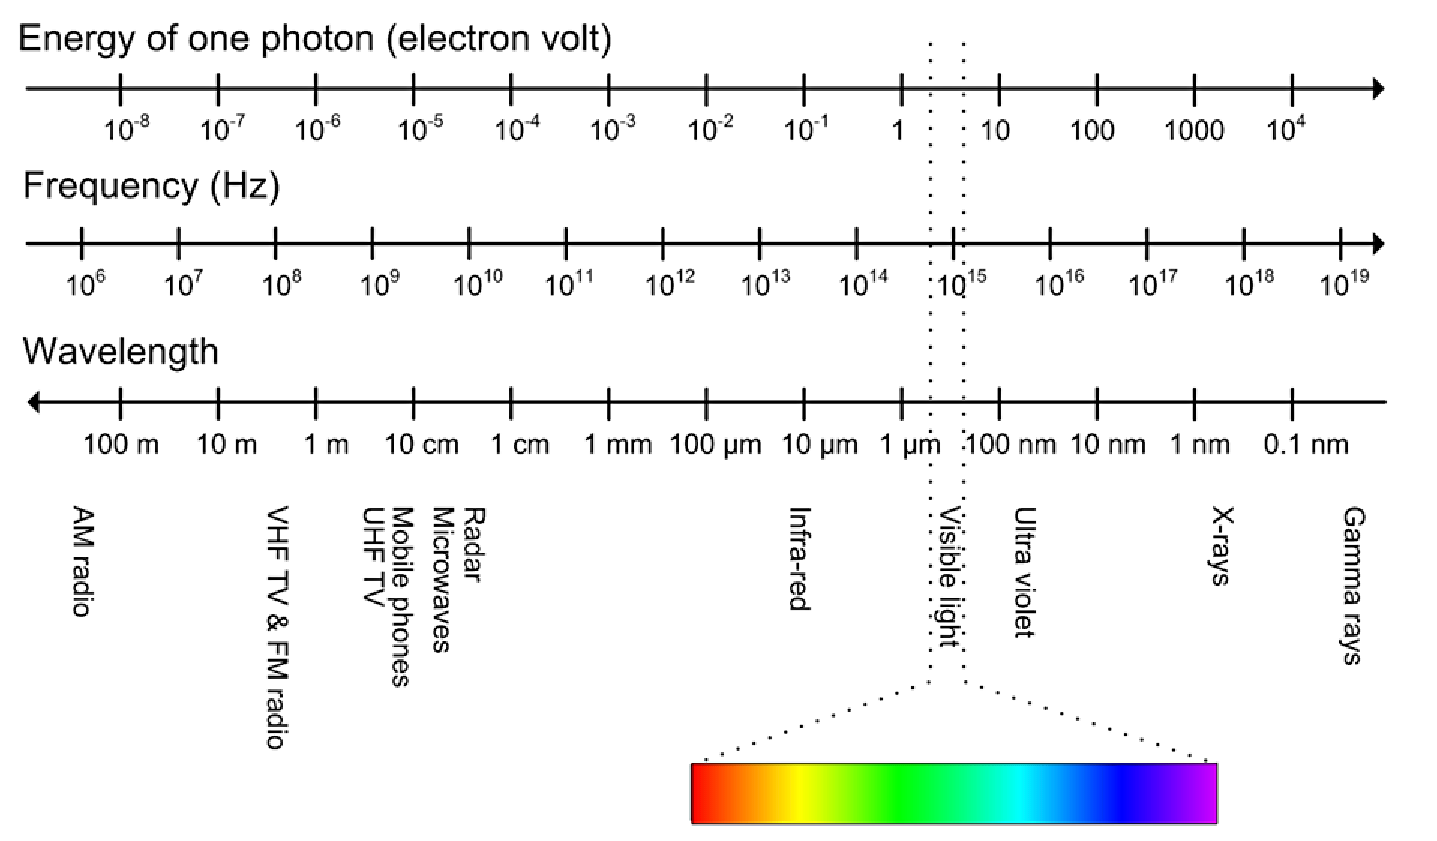
\includegraphics[width=10cm]{gfx/electromagneticSpectrum.png}
 \caption{Espectro Electromagnético \cite{electromagneticField}}
 \label{fig:spectrum}
\end{figure}

Dado que la frecuencia de trabajo mayormente utilizada en este tipo de antenas comprende la región microondas del espectro
electromagnético, el cual comprende desde los 300 MHz hasta los 300 GHz (ver figura \ref{fig:spectrum}), y dado que en dicho rango la 
opacidad de la atmósfera es casi nula (ver figura \ref{fig:atmosphere}), puede decirse, en términos generales, que dichas 
antenas poseen la capacidad de trabajar independientemente de las condiciones atmosféricas. En otras palabras, la señal casi no es 
atenuada por la atmósfera, tampoco es interferida ni por las lluvias ni por las nubes. Por ejemplo, si se usa como parte de un 
radar de apertura sintética, luego de un post procesamiento de la señal recibida, es posible obtener información sobre la 
textura del terreno y sobre los sustratos inferiores de las coberturas boscosas. Dependiendo de que longitud de onda del rango de
trabajo, se tiene de 3 cm a 30 cm de penetración.

\begin{figure}[H]
 \centering
 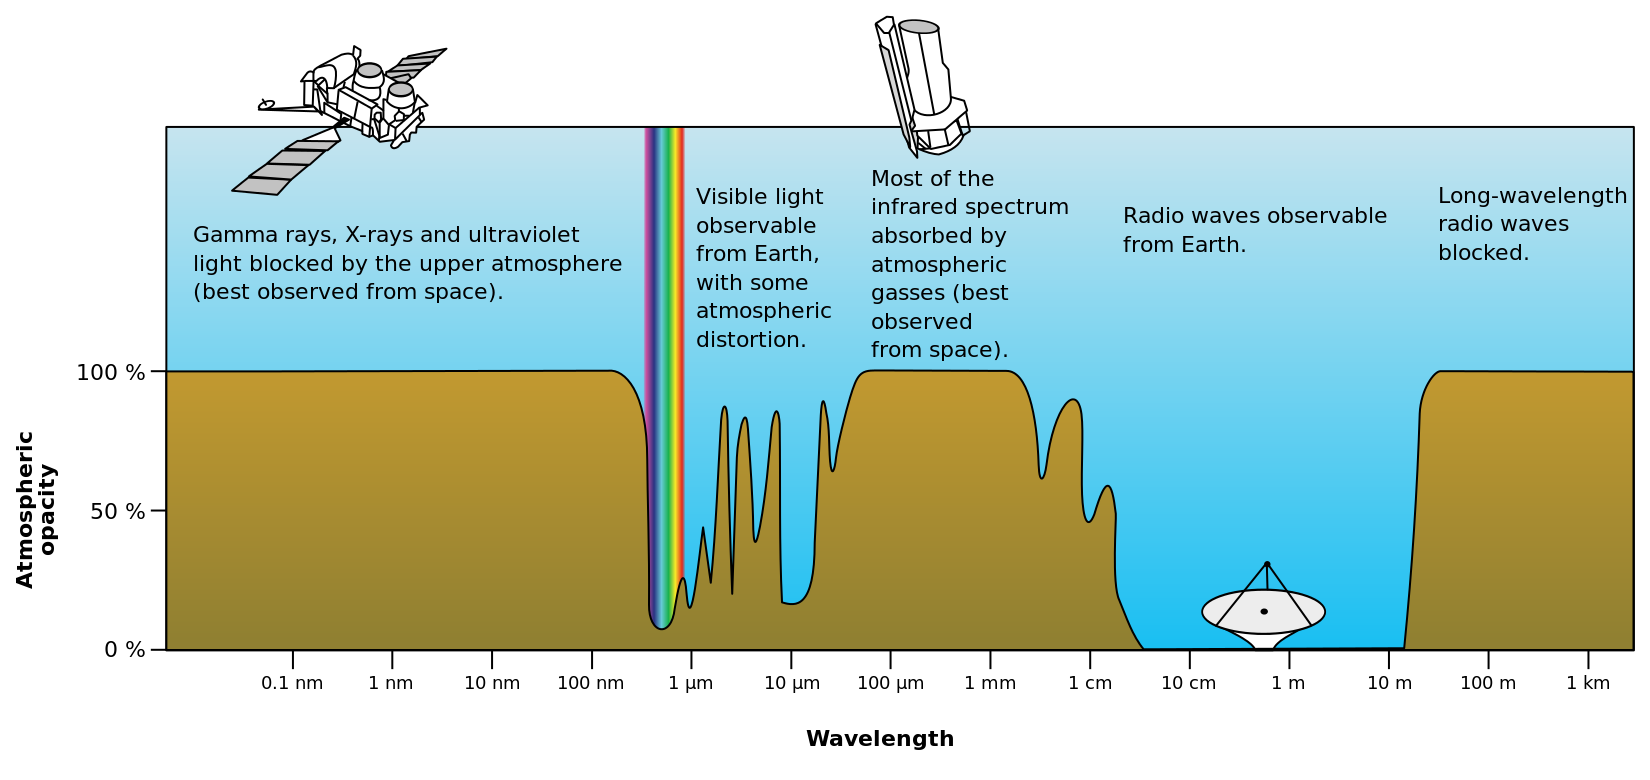
\includegraphics[width=10cm]{gfx/AtmosphericOpacity.png}
 \caption{Opacidad atmosférica vs longitud de onda \cite{electromagneticOpacity}}
 \label{fig:atmosphere}
\end{figure}

Por convención, el eje de referencia paralelo a la dirección del recorrido del satélite es llamado azimuth y la
dirección del eje perpendicular, rango. El nadir es el punto más cercano de la tierra al satélite; en otras palabras,
es el punto en la superficie terrestre que es cortado por una recta perpendicular que también corta al satélite.

La antena nunca apunta directamente hacia abajo porque, de esta forma, se perdería mucha información en rango. Al apuntar
en diagonal, y gracias a que el blanco no es puntual, el eco de la señal de la zona iluminada más cercana al nadir llega
antes al satélite que la más alejada, logrando así, tomar muestras de distintos lugares espaciados en rango (ver figura
\ref{fig:antena_ilumination}).

\begin{figure}[H]
 \centering
 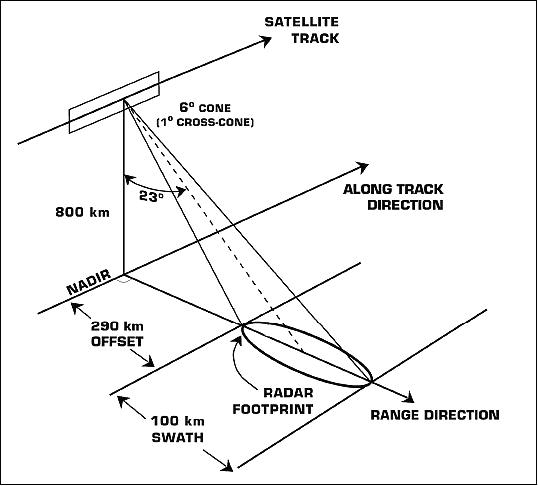
\includegraphics[width=7cm]{gfx/satellite.png}
 \caption{Footprint del satélite \cite{FootprintSatellite}.}
 \label{fig:antena_ilumination}
\end{figure}

El tamaño de la zona iluminada se llama huella. Dicho tamaño depende tanto de las dimensiones de la antena como de la
órbita del satélite o de la altura del avión en que está colocada dicha antena. Como se observa en la imagen
\ref{fig:footprint}, mientras más larga es la antena, más angosto es la huella, logrando así mejorar la resolución
espacial.

\begin{figure}[H]
 \centering
 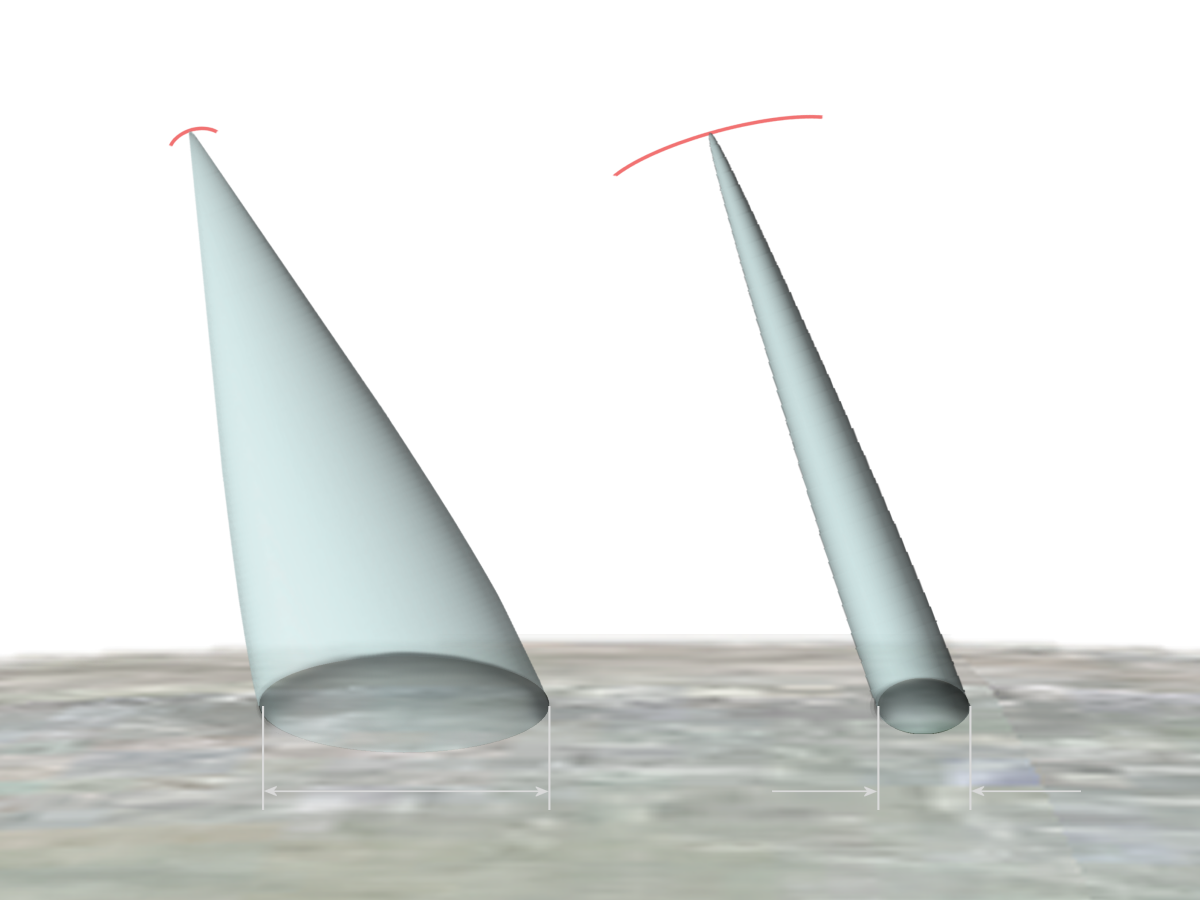
\includegraphics[width=7cm]{gfx/footprint.png}
 \caption{La huella depende del largo de la antena \cite{FootprintAntenna}.}
 \label{fig:footprint}
\end{figure}

\subsection{Composición de una antena}

Un conjunto de antena polarimétrica consta de una colección de $N$ elementos radiantes. Se asume que dichos elementos poseen el
mismos diagrama de radiación y que están orientados en el mismo sentido y dirección en un ambiente tridimensional. No es
necesario que estén espaciados regularmente ni que emitan los mismos valores de potencia y fase, pero si se asume
que todos están alimentados con la misma frecuencia de trabajo. En la figura \ref{fig:phasedArrayAntenna} se pueden observar
dos tipos de distribuciones comúnmente utilizadas.

\begin{figure}[H]
	\centering
 	\subfloat[]{
		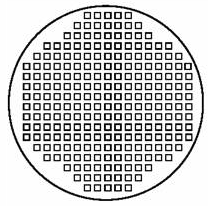
\includegraphics[width=4cm]{gfx/phasedArrayAntenna.png}}
	\subfloat[]{
		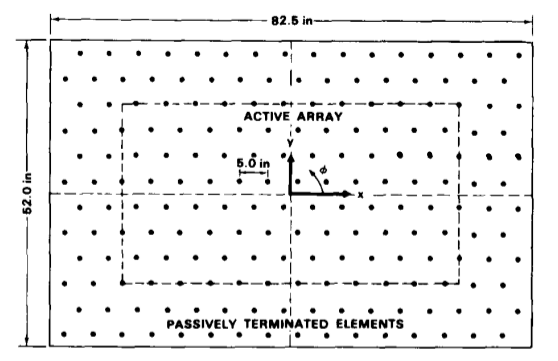
\includegraphics[width=6cm]{gfx/frontAntenna.png}}
		\caption{Conjuntos de antena: (a) Circular \cite{AntennaFront}. (b) Rectangular \cite{Aumann1989}.}
	\label{fig:phasedArrayAntenna}
\end{figure}

Este tipo de antenas está compuesto por dos bloques principales a saber: la red de distribución (o RFDN) y los elementos 
radiantes (ver figura \ref{fig:compositionAntenna}).

\begin{figure}[H]
 \centering
 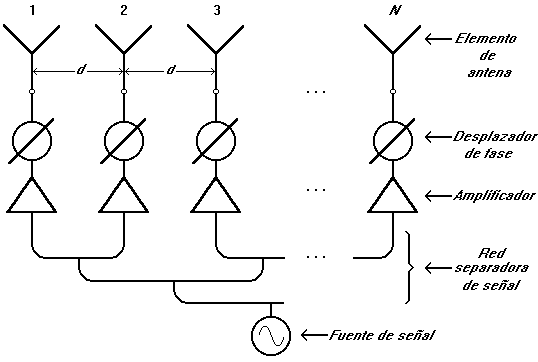
\includegraphics[width=10cm]{gfx/CompositionAntenna.png}
 \caption{Composición de un conjunto de antena}
 \label{fig:compositionAntenna}
\end{figure}

El generador puede emitir distintos tipos de modulaciones. Ej, cuadrada, chirp, senoidal, triangular, etc. Las ventajas y
desventajas de cada una se lista en el cuadro \ref{tab:modulations}

\begin{table}[H]
  \footnotesize
  \centering
  \begin{tabular}{|c|p{9cm}|}
	\hline
	\textbf{Modulación} & \textbf{Características} \\
	Cuadrada & Esta modulación es utilizada para mediciones muy precisas a cortas distancias comparando las fases de los dos
	semiciclos de la señal recibida. La desventaja es que los distintos ecos de los distintos blancos no pueden distinguirse.\\\hline
	Chirp & Es la modulación mayormente utilizada, se obtienen mediciones con las mayores distancias posibles.\\\hline
	Triangular & Con esta modulación se logra distinguir fácilmente la velocidad de la posición del blanco. \\\hline
	Escalonada & Es utilizada para mediciones de interferometría y para expandir el rango de medición sin ambig\"uedades.\\\hline
  \end{tabular}
  \caption{Características de cada modulación de la señal emitida}
  \label{tab:modulations}
\end{table}

La red de distribución, llamada RFDN, es la encargada de transmitir la señal a todos los elementos radiantes de la antena.
Dicha red posee una estructura de árbol, de forma tal, que la longitud de todos los caminos entre las hojas del mismo a
la raíz son iguale (Los nodos son los PSC y las hojas los RMs). Es necesraio que todos los caminos sean iguales para que las
señales transmitidas posean la misma fase y atenuación. Los componentes utilizados para distribuir la señal son los siguientes:

\begin{itemize}
	\item Divisor/Combinador de potencia de RF: este componente es el encargado de dividir la señal transmitida en tantos puertos 
		de salida tenga y la de sumar/combinar las potencias recibidas.
	\item Cable: este componente es el utilizado para unir el resto de los componentes.
	\item Módulo de Transmisión y Recepción: Este componente es el elemento de control de fase y atenuación de la señal emitida y
		recibida por la antena. Para la modelización realizada, se considera que hay uno por cada elemento radiante.
	\item Defasador: Este componente simplemente defasa la señal, hay uno por cada elemento radiante, se lo utiliza
		para poder calibrar la antena tanto en transmisión como en recepción, logrando así, que cada camino de transmisión/
		recepción de las hojas a la raíz defasen lo mismo. A su vez, se lo utiliza para poder direccionar el beam de la señal
		emitida.
	\item Elemento Radiante: Este componente es el emisor de la señal a transmitir y/o el receptor. En este tipo de antenas un
		RM puede cumplir una o ambas funcionalidades.
	\item Circulador: Este componente posee tres puertos y es utilizado para separar los caminos de la señal transmitida (Tx) de 
		la recibida (Rx) cuando un mismo elemento radiante posee las funcionalidades de transmisión y recepción. 
\end{itemize}

Se pueden conectar los elementos radiantes de tal forma que puedan transmitir en dos polarizaciones distintas, H y V (Ver figura
\ref{fig:polarizations}), para esto, se debe duplicar la RFDN. Haciendo uso de ambas polarizaciones se puede caracterizar
los blancos observados, dado que, cada cuerpo responde de forma distinta a cada tipo de polarización.

\begin{figure}[H]
 \centering
 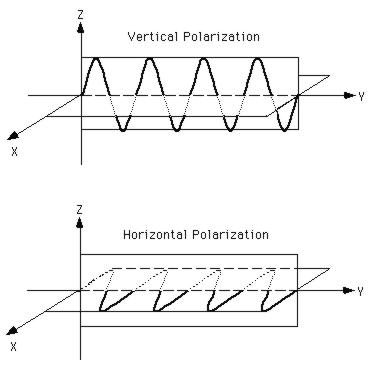
\includegraphics[width=7cm]{gfx/HAndVPolarizations.png}
 \caption{Polarizaciones verticales y horizontales}
 \label{fig:polarizations}
\end{figure}


\subsection{Diagrama de radiación de antena}

Un conjunto de antena puede armarse recursivamente, esto es, que un elemento sea, en si mismo, un conjunto. Un diagrama de antena es
un diagrama de radiación polar que resulta de reemplazar cada elemento por un radiador isotrópico. Si se asume que el diagrama de
radiación de cada elemento es idéntico al del resto, tomando una cierta incertidumbre, el diagrama de radiación total resulta de
la multiplicación de todos los diagramas de todos los elementos. Este resultado no depende de si se consideran los diagramas de
potencia o de amplitud/fase.

\begin{figure}[H]
 \centering
 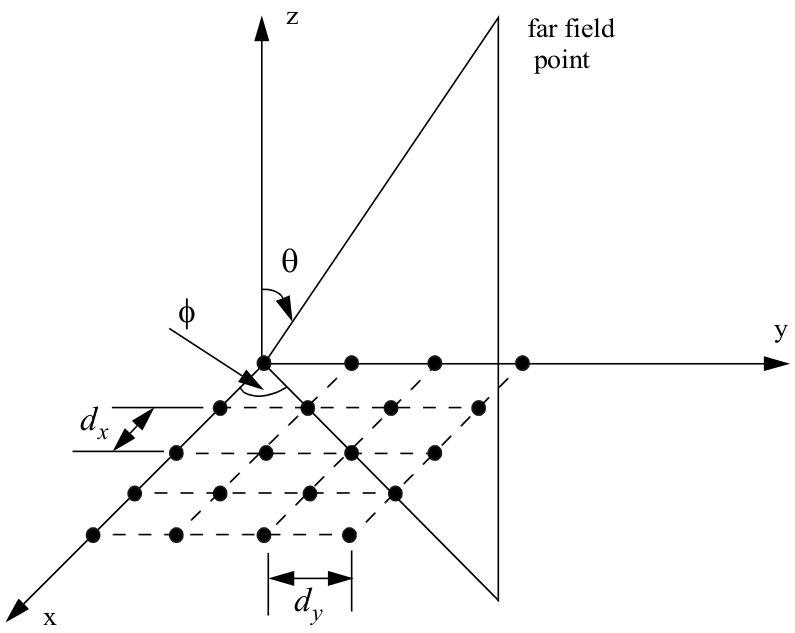
\includegraphics[width=7cm]{gfx/rectangularArrayGeometry.png}
 \caption{Conjunto de geometría rectangular \cite{Mahafza2004}}
 \label{fig:arrayGeometry}
\end{figure}

Considerese un conjunto de antena de $NxM$ elementos, como se muestra en la figura \ref{fig:arrayGeometry}, el diagrama de
radiación de campo lejano se lo calcula de la siguiente forma \cite{Mahafza2004}.

\begin{equation}
	E(\theta, \phi) = \sum_{n=0}^{N-1}\sum_{m=0}^{M-1} I_{n,m} e^{jk(d_xn\sin\phi\cos\theta + d_ym\sin\phi\sin\theta)}
\end{equation}

Donde $\theta$ corresponde al ángulo al eje x, $\phi$ corresponde al ángulo al eje z, $k$ es el número de onda y es igual
a $2\pi/\lambda$, $I_{n,m}$ es la amplitud compleja del elemento $n,m$. La figura \ref{fig:arrayPattern} muestra el diagrama de
radiación en tres dimensiones, donde el eje $Z$ (representado con colores) es la potencia radiada. A su vez, se puede apreciar 
uno de los cortes que se realizan generalmente sobre los mismos (elevacion o azimuth).

\begin{figure}[H]
 \centering
	\subfloat[]{
		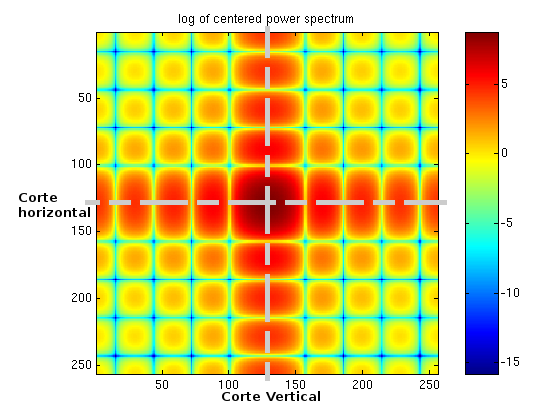
\includegraphics[width=7cm]{gfx/arrayPattern3D.png}}
 	\subfloat[]{
		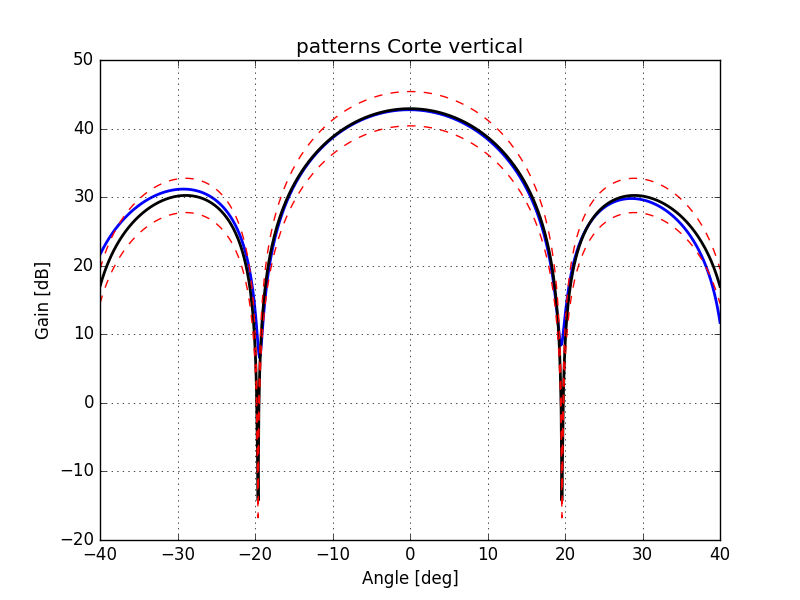
\includegraphics[width=7cm]{gfx/arrayPatternCut.png}}
	\caption{diagramas de radiación de un conjunto de antena (a) diagrama en 3 dimensiones \cite{arrayPattern} (b) corte horizontal}
 \label{fig:arrayPattern}
\end{figure}

Los tres parámetros más importantes del diagrama de radiación son la directividad, el ancho del lóbulo principal y el nivel
de los lóbulos secundarios \cite{Hsiao1985}. Es importante incrementar lo más posible la diferencia de potencia entre los 
lóbulos secundarios y el principal. Para lo cual, si se desea realizar un achicamiento de los lóbulos secundarios sin modificar 
la directividad como el ancho del lóbulo principal, es necesario incrementar el tamaño del conjunto de antena \cite{Hsiao1985}. 
Lamentablemente los errores, incertidumbres y desvíos en el comportamiento del conjunto limitan los niveles que se pueden 
obtener de los lóbulos secundarios \cite{Hsiao1985}.

A continuación se muestran gráficos representando la potencia del campo radiado, asumiendo campo lejano. La potencia decae
con la relación de $1/r$, donde $r$ es la distancia del punto de medición al elemento radiado. Se debe tomar en cuenta también
la fase con que emite el elemento y el retardo de fase que se debe a la distancia recorrida por la señal para llegar a los 
distintos lugares del espacio. Dicho retardo es expresado como $2\pi r/\lambda$, siendo $\lambda$ la longitud de onda de la 
señal emitida por el elemento radiado. Los gráficos \ref{fig:twoArrayPat} y \ref{fig:fourArrayPat} muestran las curvas de 
nivel de diagramas de radiación de potencia polar, donde los elementos radiantes están distribuidos uniformemente sobre el eje
x (eje horizontal) y emiten en fase.

\begin{figure}[H]
	\centering
	\subfloat[]{
		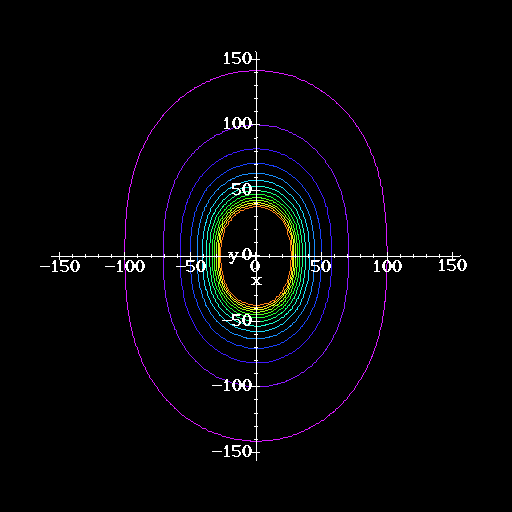
\includegraphics[width=5cm]{gfx/TwoIsoQuartDist.png}}
	\subfloat[]{
		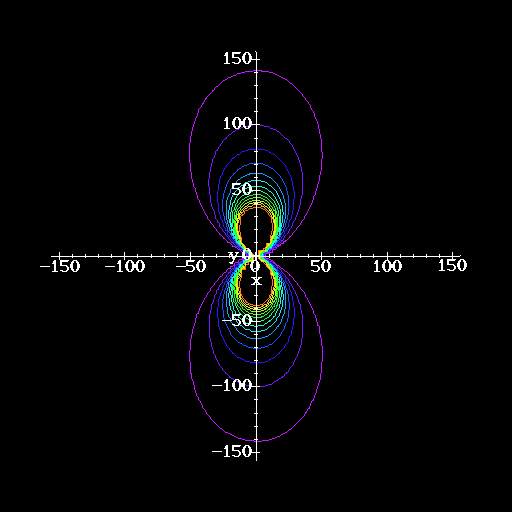
\includegraphics[width=5cm]{gfx/TwoIsoHalfDist.png}}
	\caption{Diagramas de radiación de potencia. Dos RMs con separación de: a) $1/4$ de longitud de onda, b) $1/2$ de longitud de onda}
	\label{fig:twoArrayPat}
\end{figure}

\begin{figure}[H]
	\centering
	\subfloat[]{
		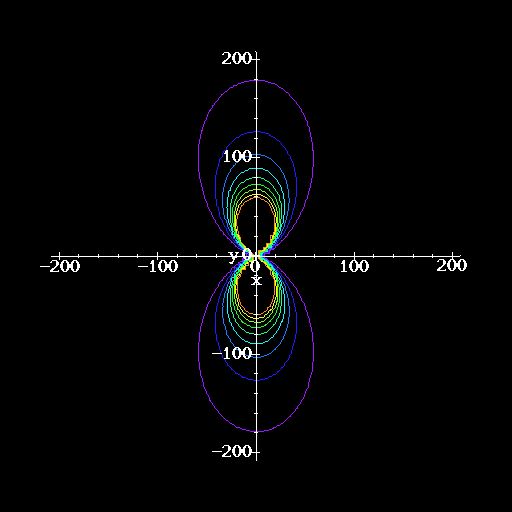
\includegraphics[width=5cm]{gfx/FourIsoQuartDist.png}}
	\subfloat[]{
		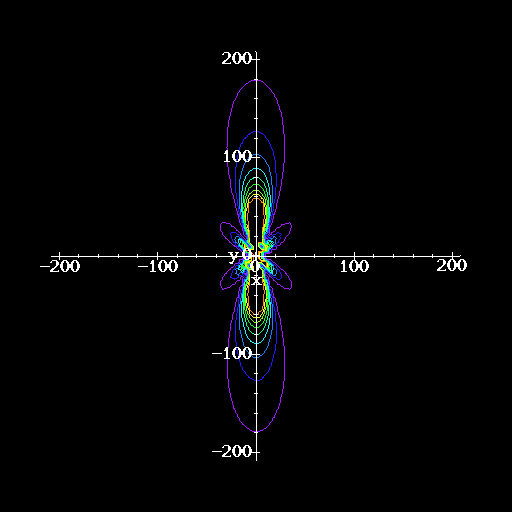
\includegraphics[width=5cm]{gfx/FourIsoHalfDist.png}}
	\caption{Diagramas de radiación de potencia. Cuatro RMs con separación de: a) $1/4$ de longitud de onda, b) $1/2$ de longitud
		de onda}
	\label{fig:fourArrayPat}
\end{figure}

Se puede observar que aumentando la cantidad de elementos radiantes, se logra que el haz principal (lóbulo principal de
potencia) sea más angosto, por lo tanto se obtenga una mayor resolución del cuerpo observado. La figura \ref{fig:directArrayPat} 
muestra que la fase con que emiten los elementos radiados modifica el apuntamiento de la antena.

\begin{figure}[H]
	\centering
	\subfloat[]{
		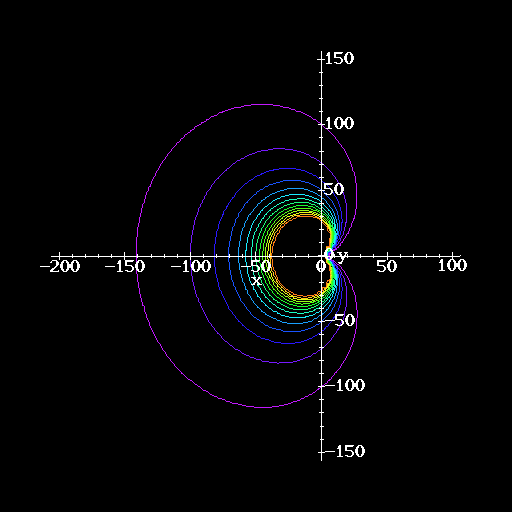
\includegraphics[width=5cm]{gfx/TwoQuarterPhase.png}}
	\subfloat[]{
		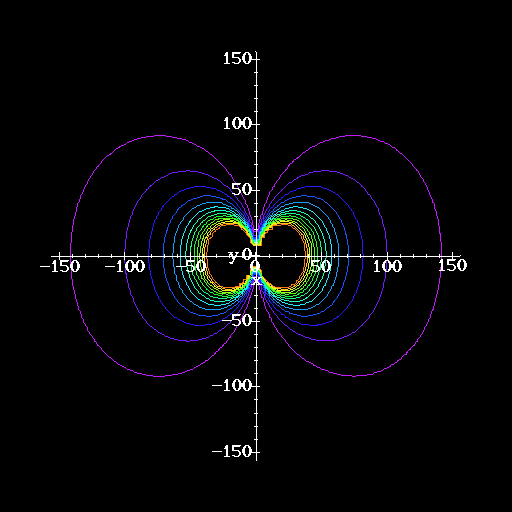
\includegraphics[width=5cm]{gfx/TwoAntiPhase.png}}
	\caption{Diagrama de radiación de potencia. Dos RMs en contrafase y con separación de: a) $1/4$ de longitud de onda. b) $1/2$ 
		de longitud de onda}
	\label{fig:directArrayPat}
\end{figure}


\subsection{Apuntamiento de una antena}\label{ssec:beamSteering}

Para que la suma de todas las señales emitidas con todos los elementos radiantes apunte a un mismo punto, es necesario que
todas las ondas lleguen al objetivo con la misma fase. Es por esto que se debe saber determinar cual es la fase individual que
debe tener cada uno de los elementos radiantes.

Como primer simplificación, se puede asumir que todas las rectas de cada uno de los elementos radiantes al punto lejano son
paralelas entre ellas. A su vez, como el camino recorrido desde cada elemento radiante al punto lejano es diferente, es
necesario calcular dicha diferencia para luego relacionarla con la fase. De esta forma, se puede retrasar la fase emitida de
los elementos más alejados al punto para que todas las señales lleguen en fase, logrando así, una onda plana.

La figura \ref{fig:beamSteering} muestra como se realiza el apuntamiento de un conjunto de antena en una sola dirección,
para la dirección perpendicular, el razonamiento es totalmente análogo.

\begin{figure}[H]
 \centering
 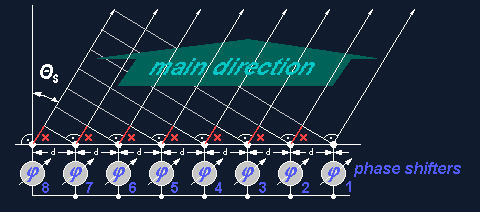
\includegraphics[width=10cm]{gfx/beamSteering.png}
 \caption{Apuntamiento con una conjunto de antena \cite{BeamSteering}.}
 \label{fig:beamSteering}
\end{figure}

Como se puede observar en la figura \ref{fig:beamSteering}, la diferencia de fase entre dos elementos consecutivos,
$\Delta\varphi$, es constante y es llamada incremento de fase \cite{BeamSteering}. Se la puede relacionar con la diferencia
de distancia que tiene que recorrer el haz emitido por cada elemento radiante. Dicha diferencia de distancia se la calcula con
la siguiente relación matemática,


\begin{equation}
	x = d\cdot \sin{\theta_s}
	\label{eq:steering}
\end{equation}

Donde $d$ es la distancia entre dos elementos consecutivos y $\theta_s$ es el apuntamiento deseado del haz emitido. Para calcular
el defasaje de una onda en una cierta distancia $x$, se debe tener en cuenta que depende de su longitud de onda.

\begin{equation}
	\dfrac{2\pi}{\Delta\varphi} = \dfrac{\lambda}{x}
	\label{eq:dist2angle}
\end{equation}

Donde $\Delta\varphi$ es el incremento de fase entre elementos radiantes, $\lambda$ es la longitud de onda transmitida.
Utilizando las ecuaciones \ref{eq:steering} en \ref{eq:dist2angle} se puede obtener el incremento de fase entre RMs contiguos 
necesario para cumplir con el apuntamiento deseado. La ecuación matemática a continuación.

\begin{equation}
	\Delta\varphi = \dfrac{2\pi\cdot d\cdot\sin{\theta_s}}{\lambda}
\end{equation}

\subsection{Calibración interna de una antena polarimétrica}

La respuesta de los componentes varía por el envejecimiento de los mismos al pasar del tiempo, por variaciones de la temperatura
de operación, el manejo imprudente de los mismos, interferencias electromagnéticas (radiadas o conducidas), etc. Dichas 
variaciones deben ser corregidas, buscando que no solo todos los caminos de recepción atenúen y defasen exactamente lo
mismo, sino que también sea un valor conocido. En transmisión el objetivo es el mismo, con la salvedad que se busca que cada
TRM trabaje en su punto de compresión (generalmente cerca de los 6dB) y que la fase de cada elemento depende del apuntamiento
deseado.

Para calibrar la antena por medio de lazos de calibración, la electrónica central se comporta como un VNA (representado en la 
figura \ref{fig:calibrationLoop}). La misma emite una señal por un canal y la compara con lo recibido en el otro canal, 
midiendo el S21 (transmisión directa) de los parámetros S de la antena. Para ello, se debe descontar a la señal recibida, la 
señal emitida. Dicha calibración determina las características de la antena para un determinado instante, si los componentes 
cambian sus características en el tiempo, se debería realizar el proceso de calibración nuevamente para obtener los nuevos 
parámetros S.

\begin{figure}[H]
 \centering
 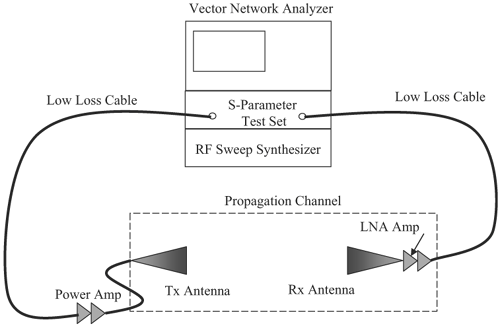
\includegraphics[width=10cm]{gfx/calibrationLoop.png}
 \caption{Lazo de calibración utilizando un VNA \cite{Reed2012}.}
 \label{fig:calibrationLoop}
\end{figure}

La figura \ref{fig:nonCalPattern} muestra la comparación de dos diagramas de radiación de antena, uno calibrado e ideal y el
otro sin calibrar. Se puede observar como los niveles de los lóbulos secundarios y el ancho del lóbulo principal se incrementan.

\begin{figure}[H]
 \centering
 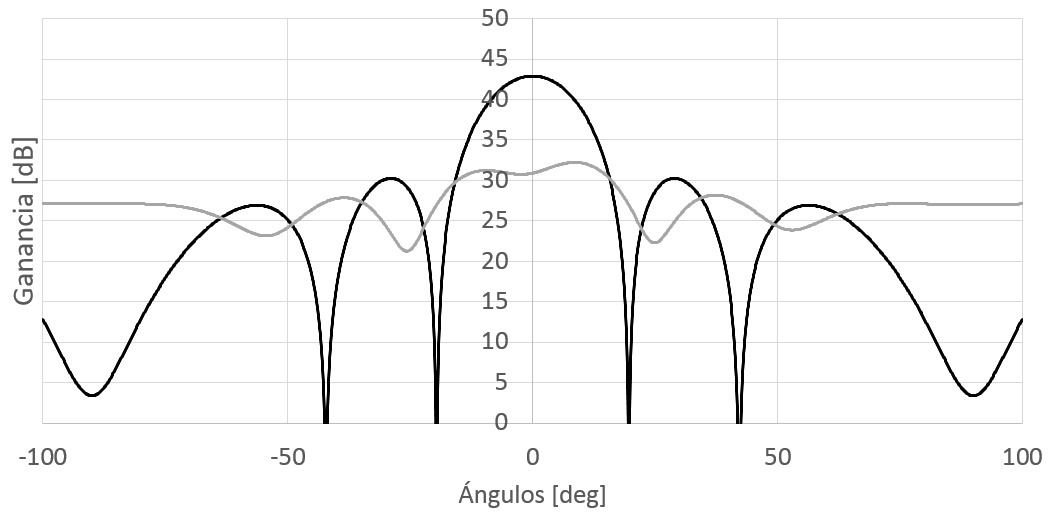
\includegraphics[width=10cm]{gfx/nonCalPattern.png}
 \caption{Diagrama de radiación de antena calibrado vs no calibrado.}
 \label{fig:nonCalPattern}
\end{figure}

\section{Parámetros S de cada componente}

Los componentes que son ideales, se los trata como si estuviesen perfectamente adaptados, logrando así que los coeficientes
de reflexión sean nulos, esto es $S_{11} = S_{22} = 0$. Para mayor información sobre que son los parámetros S ver el apéndice
\ref{sc:appendixSParam}.

\subsection{Elemento Radiante (RM)}

El elemento radiante es un módulo de un único puerto y es pasivo, por lo tanto el parámetro S que lo define es $S_{11}$ y su
valor varía entre -1 y 1.

\begin{itemize}
	\item Cortocircuito ideal: $S_{11} = -1$
	\item Conexión ideal: $S_{11} = 0$
	\item Circuito abierto ideal: $S_{11} = 1$
\end{itemize}

Los casos de cortocircuito y circuito abierto son casos de falla del módulo radiante. Cualquier otro valor intermedio implica
una desadaptación de impedancias.

\subsection{Cable ideal}
Un cable se comporta como una línea de transmisión, y su matriz es la siguiente

$$
\mathbf{S} = \begin{pmatrix} 0 & e^{-\gamma l}\\e^{-\gamma l} & 0\end{pmatrix}
$$

Donde $\gamma = \alpha + j\beta$ es una constante de propagación compleja. $\alpha$ es la atenuación de la línea en [neper/m]
y $\beta = 2\pi/\delta$ con la longitud de onda $\delta$. Para una línea sin pérdidas se obtiene $|S_{21}| = 1$

\subsection{Desplazador de fase ideal}


$$
\mathbf{S} = \begin{pmatrix} 0 & e^{-j\phi_{12}}\\e^{-j\phi_{21}} & 0\end{pmatrix}
$$

Un defasador recíproco posee $\phi_{12} = \phi_{21}$.

\subsection{Atenuador ideal}

$$
\mathbf{S} = \begin{pmatrix} 0 & e^{-\beta}\\e^{-\alpha} & 0\end{pmatrix}
$$

Si el atenuador es recíproco, $\alpha = \beta$. El factor de atenuación, $\alpha$, está en neper. La atenuación en decibeles
viene dado por $A = '20\log_{10}(S_{21})$, $1N = 8.686dB$.


\subsection{Amplificador ideal}

$$
\mathbf{S} = \begin{pmatrix} 0 & 0\\G & 0\end{pmatrix}
$$

Con $G > 1$.


\subsection{Módulo de transmisión recepción ideal}

Dicho componente está compuesto por un defasador ideal junto a un amplificador. Es un componente de tres puertos, el primero 
puede transmitir o recibir señal, el segundo solamente transmitir y el tercero recibir. Su matriz de parámetros S es la siguiente.

$$
	S_{PSC} = \begin{pmatrix} 0&0&Ge^{-j\phi_{13}} \\ Ge^{-j\phi_{21}}&0&0 \\ 0&0&0\end{pmatrix} 
$$

Este componente se lo puede configurar para unir el primer puerto con el segundo o con el tercero por medio de un interruptor, 
por lo tanto no se lo puede utilizar para transmitir y recibir a la vez. 

\begin{figure}[H]
 \centering
 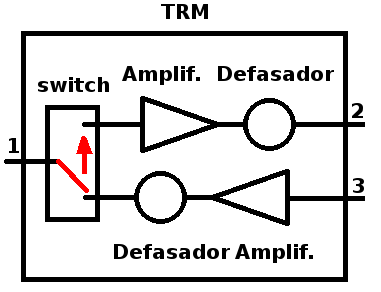
\includegraphics[width=4cm]{gfx/trm.png}
 \caption{módulo de transmisión/recepción}
 \label{fig:trm}
\end{figure}


\subsection{Circulador ideal}

El circulador ideal es sin pérdidas y adaptado en todos sus puertos. La señal entrante por un puerto es exclusivamente
transmitida al puerto siguiente en el sentido de la flecha.

\begin{figure}[H]
 \centering
 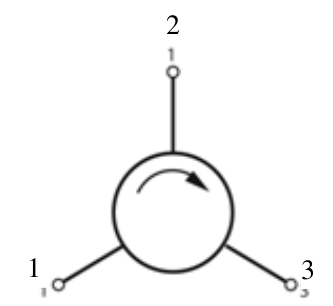
\includegraphics[width=4cm]{gfx/circulator.png}
 \caption{circulador de 3 puertos}
 \label{fig:circulator}
\end{figure}

La matriz de parámetros S es como sigue.

$$
\mathbf{S} = \begin{pmatrix} 0 & 0 & 1\\1 & 0 & 0\\0 & 1 & 0\end{pmatrix}
$$


\subsection{Divisor/Combinador de potencia en RF (PSC)}

El tipo de PSC modelado consiste en una red recíproca y adaptada en todos sus puertos, pero con pérdidas. Puede ser un
componente de 3 o más puertos. A continuación se muestra la matriz de parámetros S genérica para una red de n puertos
(matriz de nxn).

$$
\mathbf{S} = \begin{pmatrix} 0 & \dfrac{1}{n-1} & ... & \dfrac{1}{n-1}\\
							 \dfrac{1}{n-1} & 0 & ... & \dfrac{1}{n-1}\\
							 ... & ... & ... & ... \\
							 \dfrac{1}{n-1} & \dfrac{1}{n-1} & ... & 0 \end{pmatrix}
$$

\subsection{Acoplamientos mútuos}

El acoplamiento mutuo entre módulos radiantes es modelizado con el mismo comportamiento al de un cable, pero con las
propiedades de atenuación y defasaje de una onda en el vacío. Las cuales son:

\begin{equation}
	S12 = S21 = \dfrac{e^{-j\dfrac{\pi}{\lambda}r}}{4\pi r^2}
\end{equation}

siendo r la distancia recorrida por la señal. La matriz de parámetros S resulta,

$$
\mathbf{S} = \begin{pmatrix} 0 & \dfrac{e^{-j\dfrac{\pi}{\lambda}r}}{4\pi r^2}\\\dfrac{e^{-j\dfrac{\pi}{\lambda}r}}{4\pi r^2} & 0\end{pmatrix}
$$

\section{Ejemplo parámetros S}

En esta sección se ejemplifica el armado de las matrices de parámetros S de la antena en una sola polarización desde el punto 
de transmisión a cada elemento radiante. Se asume que se tiene una antena de dos elementos radiantes con la configuración de 
RFDN de la figura \ref{fig:antennaS}. Dicha figura muestra solamente la red de distribución en una sola polarización, para la 
otra polarización, este esquema se repite.

\begin{figure}[H]
 \centering
 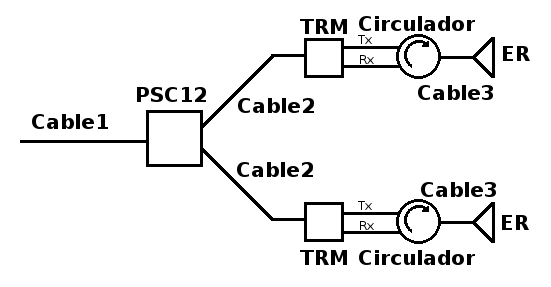
\includegraphics[width=9cm]{gfx/RFDN.png}
 \caption{RFDN para una polarización del esquema de antena.}
 \label{fig:antennaS}
\end{figure}

La tabla \ref{tab:componentSParameters} muestra la cantidad de puertos que posee cada componente y la conexión de cada puerto.

\begin{table}[H]
  \footnotesize
  \centering
  \begin{tabular}{|c|c|p{6cm}|}
	\hline
	\textbf{Componente de Antena} & \textbf{Cantidad de puertos} & \textbf{Notas} \tabularnewline \hline
	cable1 &  2 & \tabularnewline \hline
	\multirow{3}{*}{PSC12} & & Puerto1: conexión cable1 \tabularnewline
	 & 3 & Puerto2: conexión Cable2 (superior) \tabularnewline
	 & & puerto3: conexión Cable2 (inferior) \tabularnewline \hline
	Cable2 & 2 & \tabularnewline \hline
	\multirow{3}{*}{TRM} & & Puerto1: conexión cable2 \tabularnewline
	 & 3 & puerto2: conexión Tx \tabularnewline
	 & & puerto3: conexión Rx \tabularnewline \hline
	\multirow{3}{*}{Circulador} & & Puerto1: conexión Tx \tabularnewline
	 & 3 & puerto2: conexión Cable3 \tabularnewline
	 & & puerto3: conexión Rx \tabularnewline \hline
	Cable3 & 2 & \tabularnewline \hline
	RM & 1 & \tabularnewline \hline
  \end{tabular}
  \caption{Propiedades físicas de cada componente de una antena}
  \label{tab:componentSParameters}
\end{table}

Para la obtención de la respuesta del sistema desde el punto de transmisión/recepción a cada elemento radiante se debe
transformar las matrices de 3 puertos en matrices de 2 puertos. Para ello se deben determinar los puertos de conexión utilizados
para la obtención de dicha matriz asumiendo que se desea obtener la respuesta del sistema de transmisión del elemento radiante
2 (camino en rojo de la figura \ref{fig:antennaSLoop}).

\begin{figure}[H]
 \centering
 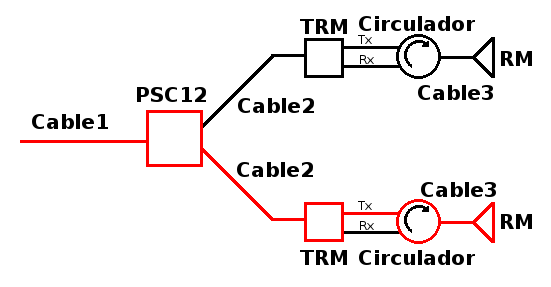
\includegraphics[width=9cm]{gfx/RFDNLoop.png}
 \caption{RFDN para una polarización del esquema de antena. En rojo, cascada de redes de dos puertos.}
 \label{fig:antennaSLoop}
\end{figure}

Como los puertos utilizados por el PSC en el camino rojo de la figura \ref{fig:antennaSLoop} son el 1 y 3, la conversión de
parámetros S resulta ser,

$$
	S_{PSC} = \begin{pmatrix} S11&S12&S13 \\ S21&S22&S23 \\ S31&S32&S33\end{pmatrix} \Rightarrow
	S_{PSC_{13}} = \begin{pmatrix} S11&S13 \\ S31&S33 \end{pmatrix}
$$

Los puertos utilizados por el TRM como el circulador son el 1 y 2, por lo tanto, la conversión de ambos parámetros S resulta
equivalente.

$$
	S_{TRM} = \begin{pmatrix} S11&S12&S13 \\ S21&S22&S23 \\ S31&S32&S33\end{pmatrix} \Rightarrow
	S_{TRM_{12}} = \begin{pmatrix} S11&S12 \\ S21&S22 \end{pmatrix}
$$

$$
	S_{Circulador} = \begin{pmatrix} S11&S12&S13 \\ S21&S22&S23 \\ S31&S32&S33\end{pmatrix} \Rightarrow
	S_{Circulador_{12}} = \begin{pmatrix} S11&S12 \\ S21&S22 \end{pmatrix}
$$

Como se desea caracterizar la respuesta de una cascada de redes de dos puertos, se transforman todas las matrices de cada
componente a parámetros T (ver ecuaciones \ref{eq:s2t}), se multiplican todas las matrices como se muestra en la ecuación
\ref{eq:cascade} i luego, la matriz resultante se la vuelve a convertir a parámetros S (ver ecuaciones \ref{eq:t2s}).

$$
\begin{aligned}
	S_i &\Rightarrow T_i \\
	T_{in,rm2} &= T_{Cable1}T_{PSC_{13}}T_{Cable2}T_{TRM_{12}}T_{Circulador_{12}}T_{Cable3}T_{RM}\\
	T_{in,rm2} &\Rightarrow S_{in,rm2}
\end{aligned}
$$

Para el caso de querer caracterizar la respuesta inversa de la antena (desde el elemento radiante al receptor) del mismo camino
mostrado en rojo de la figura \ref{fig:antennaSLoop}, el procedimiento es el mismo, salvo que se utilizan los puertos 2 y 3 del
circulador y los puertos 1 y 3 del TRM.

$$
	S_{TRM} = \begin{pmatrix} S11&S12&S13 \\ S21&S22&S23 \\ S31&S32&S33\end{pmatrix} \Rightarrow
	S_{TRM_{13}} = \begin{pmatrix} S11&S13 \\ S31&S33 \end{pmatrix}
$$

$$
	S_{Circulador} = \begin{pmatrix} S11&S12&S13 \\ S21&S22&S23 \\ S31&S32&S33\end{pmatrix} \Rightarrow
	S_{Circulador_{23}} = \begin{pmatrix} S22&S23 \\ S32&S33 \end{pmatrix}
$$

Se vuelven a realizar los pasos de cascada de parámetros T y conversión a parámetros S de la matriz resultante. Pero, como
dicho resultado sigue siendo desde el receptor al módulo radiante, se deben reacomodar los elementos de la matriz

$$
	S_{out,rm2} = \begin{pmatrix} S11&S12 \\ S21&S22\end{pmatrix} \Rightarrow
	S_{rm2, out} = \begin{pmatrix} S22&S21 \\ S12&S11 \end{pmatrix}
$$
